\section{Eficiência Energética}
\par O entendimento de eficiência energética se torna necessário para entender as escolhas feitas para o projeto, assim como a implantação da tecnologia de Smart Grid e os meios alternativos de produção de energia.
\par Temos como eficiente qualquer coisa a qual funciona de acordo com as normas e com o mínimo de erros. Ao projetar o que quer que seja, devemos levar em consideração variáveis que vão além dos nossos objetivos. Tomemos como exemplo uma lâmpada: a incandescente tem o mesmo objetivo da fluorescente, iluminar o ambiente, entretanto a incandescente transformam 4\% da energia elétrica em luz e os outros 96\% em energia térmica, percebemos assim sua ineficiência, pois boa parte do recurso foi desperdiçado. Já nas fluorescentes, a relação entre produção de luz-calor respectivamente é de 20\% e 80\%, sendo de fato mais eficientes.
\par De acordo com o Plano Nacional de Eficiência Energética (PNEf), eficiência energética é o conjunto de ações de diversas naturezas que culminam na redução de energia necessária para atender as demandas da sociedade por serviços de energia. Tem com objetivo, em síntese, atender às necessidades da economia com menor uso de energia primária e, portanto, menor impacto na natureza.
\par No kit para tornar uma casa inteligente estarão inclusas ações básicas que tornam uma casa energeticamente eficiente, como utilização da energia solar como principal fonte extra de energia, além de pacotes adicionais de implementações que proporcionam um maior aproveitamento dos recursos disponíveis, melhorando assim a eficiência energética da casa e possibilitando que o consumidor escolha quais pacotes adicionais ele quer contratar, além de recomendações feitas por forma de consultoria visando uma melhoria do consumo e objetivando, assim, minimizar os gastos energéticos e, consequentemente, o impacto financeiro.

\subsection{Consumo de Energia}
\par De acordo com os dados coletados no Anuário Estatístico de Energia Elétrica de 2015, a média de consumo de uma residência no Distrito Federal, dos anos de 2011 à 2015, está em torno de 180,0 kWh/mês, porém, esses dados não levam em consideração o tamanho da habitação ou a quantidade de moradores. Além disso, por ser uma média, não considera a classe social da família, aspecto que influencia muito no gasto de energia residencial.
\par Como nosso público alvo são famílias com uma capacidade econômica considerável, foi feita uma estimativa do consumo energético de uma casa de classe média alta, levando em consideração os equipamentos e eletrodoméstico que a casa possui, bem como o tempo de uso mensal de cada dispositivo somando ainda o consumo que será acrescentado pela automação e resultando em um consumo de aproximadamente 960 KWh/mês.

\subsection{Fonte de energia da casa}
\par No projeto, para uma maior autonomia da casa, trabalha-se tanto com a energia fornecida comumente, como também com energia de fontes renováveis, que poderão ser implantadas posteriormente. A energia fornecida dita comum são as providas por empresas de distribuição de energia, como CEB e Light, enquanto as fontes de energia renováveis são aquelas que utilizam de recursos renováveis para a geração de energia elétrica.
\par Hoje já existem diversas formas de produzir energia a partir de recursos renováveis, no entanto, a maioria são aplicadas para produção de energia elétrica em grande quantidade. Numa escala residencial, o sistema mais utilizado é a produção de energia a partir de placas solares, pelo fato da alta incidência de raios solares no Brasil. Além disso, a instalação de sistemas de captação de energia solar fotovoltaica é fácil e rápida, por isso é chamada de \textit{plug-and-play} e pode-se utilizar a área do telhado para sua instalação. Sua instalação interfere muito pouco no sistema elétrico já existente no imóvel, além de servir de acordo com as necessidades da família. Como o sistema é modular, pode-se instalar um número X de painéis e, caso necessário, mais painéis poderão ser instalados no futuro sem grandes dificuldades, desde que a casa possua espaço disponível.
\par Além disso, o investimento inicial na compra de equipamentos para captação de energia solar é rapidamente recuperado por meio da economia gerada e os custos de manutenção são mínimos. Além disso, no caso da energia solar, a vida útil dos painéis é de 40 anos, o que representa um investimento rentável e duradouro. Por esses fatores, para a residência estudada, optamos em adotar o sistema de placas solares como nossa fonte extra de energia.

\subsection{Como será a utilização da energia solar}
\par Para a utilização da energia provinda das placas será utilizado o sistema \textit{on-grid}, ou sistema fotovoltaico conectado à rede, o qual possibilita a utilização da energia tanto produzida pelas placa solares quanto a própria energia da rede elétrica da concessionária. Foi escolhido esse sistema pelo fato de não necessitar de dispositivos de armazenamento, pois toda energia produzida em excedente é injetada na rede e convertido em créditos de energia, que podem ser utilizados em momentos onde a demanda é maior que a produção.
\par O sistema \textit{on-grid} trabalha em paralelo com a rede pública de distribuição de energia elétrica, ou seja, opera da mesma forma que uma usina elétrica convencional. A diferença está em sua pequena potência, se comparada a uma grande central de produção. Após a instalação e funcionamento, toda a energia gerada é transformada em corrente alternada, por um inversor, para assim ser direcionada para um medidor bidirecional e utilizada pelo no quadro geral da casa e, caso haja, o excedente é injetado na rede.
\par Esse tipo de sistema é regulamentado pela Resolução Normativa nº. 482 da Agência Nacional de Energia Elétrica (ANEEL), de 17 de abril de 2012, que é o que define o mecanismo de compensação de energia. Para a instalação do sistema conectado é necessário solicitar a autorização da distribuidora, mediante a apresentação de um projeto elétrico, um memorial descritivo e outros documentos que comprovem que o sistema segue as normas vigentes. Ainda, segundo a norma, para fins de compensação, a energia ativa injetada no sistema de distribuição pela unidade consumidora será cedida a título de empréstimo gratuito para a distribuidora, passando a unidade consumidora a ter um crédito em quantidade de energia ativa a ser consumida por um prazo de 60 (sessenta) meses.
\par Para suprir a demanda da casa que foi escolhida para aplicar o projeto, com consumo de cerca de 960 KWh/mês, são necessárias cerca de 28 placas de 320 Watts de potência. Com isso daria para suprir toda a demanda energética da casa. Nos dias nublados em que as placas possam não suprir a demanda da casa, será utilizada a energia elétrica da rede de distribuição. Contudo, mesmo o sistema solar fotovoltaico suprindo todo o consumo de energia elétrica da casa, o valor monetário da conta de luz não chega a zero, pois a distribuidora cobra uma taxa mínima, chamada de custo de disponibilidade, referentes a impostos, encargos setoriais, transmissão pelas usinas e distribuição pela distribuidora, que, no caso de Brasília, é a CEB.

\subsubsection{Dimensionamento do sistema fotovoltáico}
\par Segundo \textit{Lewton Burity Verri}, uma casa contendo quatro pessoas, sendo sua renda referente a de classe média alta, o consumo gira em torno de 39.600KW/h ao ano.
\par Para o consumo total da casa por mês, calculamos e usamos como base 956,2 kWh. Como o gasto de energia da casa é maior que a média nacional, o sistema demandará um poder de geração também maior.
\par O consumo foi baseado na tabela da Figura \ref{fig:dimensionamento}, com um adicional de segurança e para a prevenção de possíveis quedas de energia.

\begin{figure}[!h]
\label{fig:dimensionamento}
\centering
\caption{Dimensionamento do Consumo da casa}
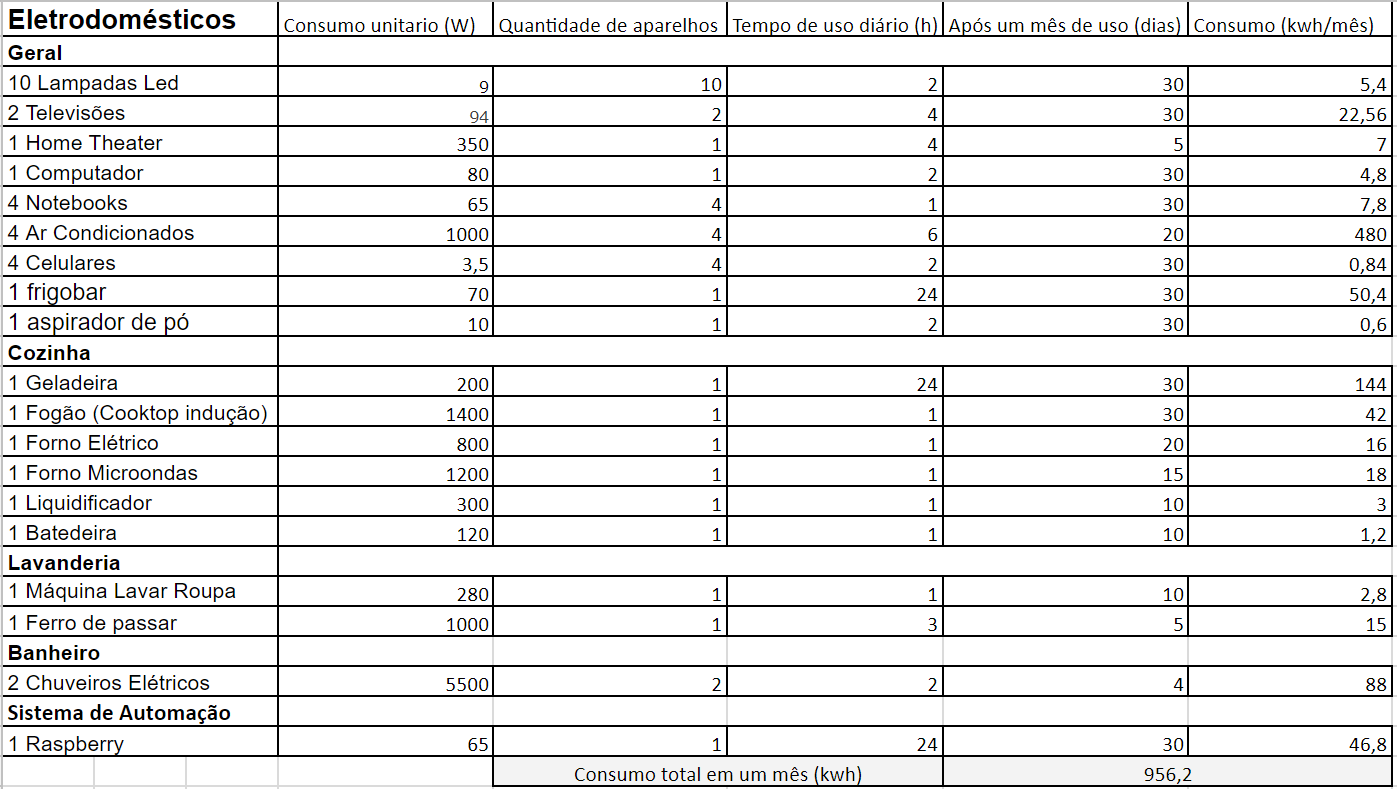
\includegraphics[width=\textwidth]{figuras/dimensionamento_consumo}
\end{figure}

\subsubsection{Painéis solares}
\par Os painéis escolhidos para a geração foram os Canadian CSI CS6U-320P. Sua potência de pico é de 320 (Wp) sendo um dos painéis com maior potência e de fácil acesso do mercado atual. No sistema em questão, será necessário o uso de 28 unidades do painel.

\begin{figure}[!h]
\centering
\caption{Canadian 320 Wp}
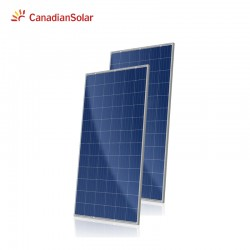
\includegraphics[width=5cm]{figuras/paineis_solares}
\end{figure}

\subsubsection{Inversor}
\par O inversor é o responsável para a conversão da corrente contínua que os painéis produzem para a corrente alternada, tipo de corrente padrão da casa. Contando que são 28 paineis de 320Wp, então o sistema fica com aproximadamente 9 kW de potência total. O inversor dimensionado então foi o Inversor Fronius Primo 8.2-1 (8.200W).
\par Todos os inversores trabalham numa margem de mais ou menos 25\% da sua potência ideal, portanto é totalmente seguro implementá-lo na casa.

\begin{figure}[!h]
\centering
\caption{Inversor Fronius 8,2 kW}
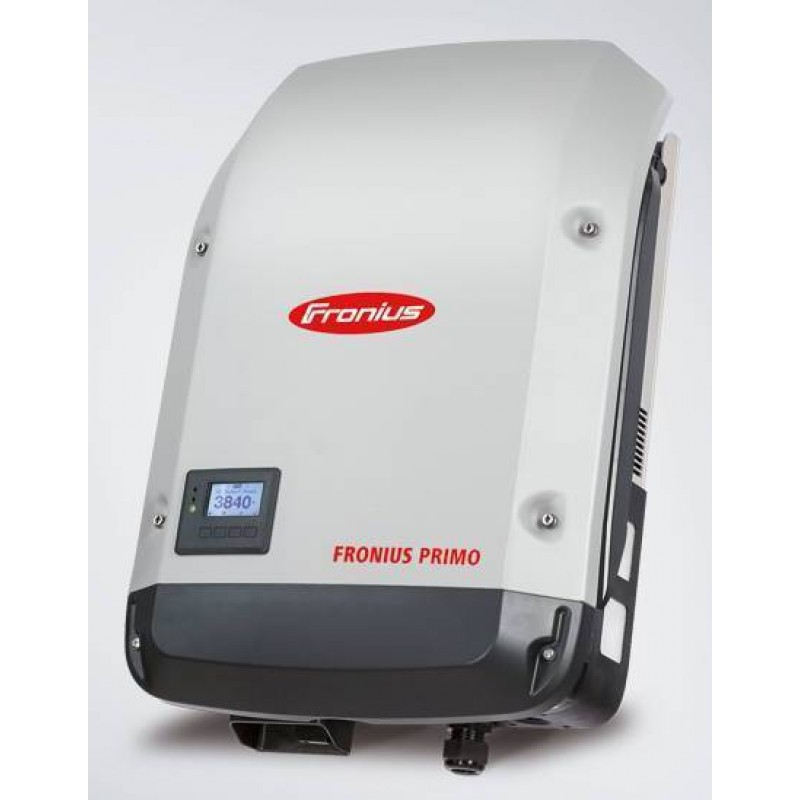
\includegraphics[width=5cm]{figuras/inversor}
\end{figure}

\subsubsection{Energia Consumida x Energia Gerada}
\par É importante salientar que cada mês do ano, a variação entre energia consumida e gerada existe, isso devido à incidência solar que também varia consideravelmente durante o ano. Para melhor ilustrar essa variação, segue o gráfico gerado:

\begin{figure}[!h]
\centering
\caption{Consumo e Energia Gerada}
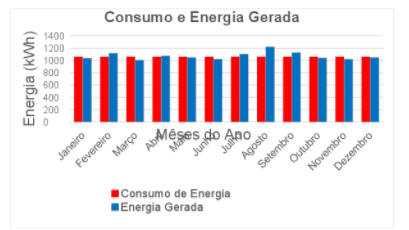
\includegraphics[width=\textwidth]{figuras/consumo_energia_gerada}
\end{figure}

\subsection{Dimensionamento do sistema crítico}
\par No projeto também consta um sistema a parte do On-Grid que alimenta a casa normalmente, sendo voltado para quando houver surtos na rede elétrica ou quedas indesejadas. Em todos esses sistemas, será utilizado os seguintes equipamentos:

\subsubsection{Bateria}
\par A bateria ideal para estes cenários que foi escolhida será uma bateria de 115ah/12V, sendo compreendida uma autonomia de 2 a 3 horas de duração para os equipamentos em questão.

\begin{figure}[!h]
\centering
\caption{Bateria}
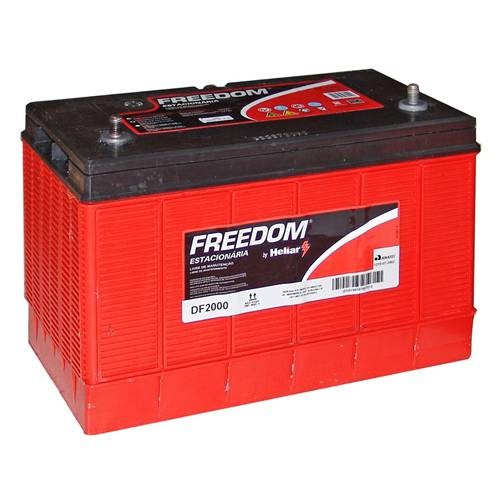
\includegraphics[width=5cm]{figuras/bateria}
\end{figure}

\subsubsection{Fonte para a bateria}
\par Foi pensado também num carregador para a bateria estacionária em questão, sendo utilizado somente para carregá-la após a queda, considerando uma queda rápida de 2 a 3 horas.

\begin{figure}[!h]
\centering
\caption{Fonte para bateria}
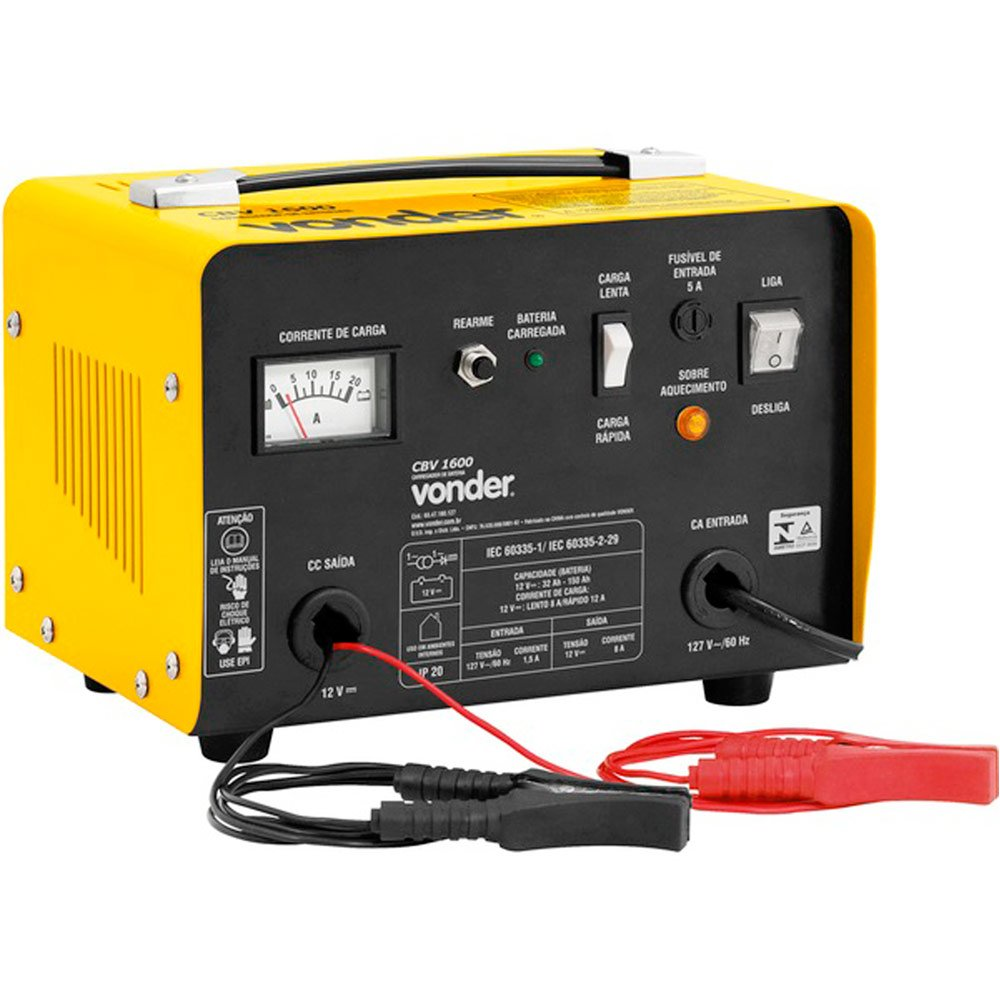
\includegraphics[width=5cm]{figuras/fonte}
\end{figure}

\subsection{Funcionamento/Automação}
\par Para que seja realizada a automação deste sistema, ou seja, o processo de mudança de fonte de energia para não atrapalhar a alimentação da central SmartGrid, será necessário um sensor chamado de sensor de tensão.
\par Ele é necessário pois a central é inicialmente ligada à fonte principal de energia da casa (sistema fotovoltaico On-Grid) e quando ocorre um surto, a rede não é capaz de fornecer essa energia. Então é nesse momento que o sensor de tensão é acionado e a fonte de alimentação da central é alternada para a energia que o banco de baterias, junto com o inversor, fornece.
\par O sensor é um componente eletrônico bem simples e pode ser controlado por um Arduíno. Ele consegue detectar se está chegando ou não uma certa tensão em seu circuito e, com o sistema já montado, ele manda a informação para o arduíno que realiza a troca de sistema.

\subsection{Pacotes Adicionais}

\subsubsection{Reutilização da água}
\par Com a aquisição desse pacote, será possível promover a reutilização das águas consumidas em algumas partes da casa, intituladas como águas cinzas. As águas cinzas são aquelas descartadas nas lavagens de roupas, lavatórios de banheiro e chuveiros. Esse tipo de água não contém tantos componentes prejudiciais ao ambiente e a saúde, como as águas negras, derivadas dos sanitários e das cozinhas, pois possuem uma alta concentração de matéria orgânica e de óleos presente no efluente.

\textbf{Reuso}
\par A falta de legislação afeta muito na questão do desenvolvimento no processo de reuso, então não existe uma padronização no tratamento.
\par Mesmo que o uso das águas seja para fins não potáveis o manual do IPT aconselha o tratamento com água sanitária e somente reutiliza-lás nas lavagens de carros, irrigação de jardins e descargas, evitando ao máximo o contato com a água.

\textbf{Filtragem}
\par Como os serviços oferecidos pela equipe serão em kits, reutilizar a água do banheiro se tornou inviável, pois necessitaria de uma pequena reforma na casa, o que já não entra no serviço. Assim, será utilizado apenas um filtro, que será instalado na parte da lavanderia da casa, acoplado à máquina de lavar onde passará por uma etapa de filtragem contendo cloro para a limpeza parcial da água, como pede a legislação (NBR 13969 de 1997) para ser utilizada na limpeza dos quintais, garagens e irrigação das plantas. O filtro será um adicional do kit vendido e tem como benefício principal a diminuição de no mínimo de 50\% no consumo de água. Será utilizado o filtro Cisterna Vertical Modular (1050 litros) com filtro Cinza.  O custo gira em torno R\$1.900,00 a R\$ 2.198,00.

\subsubsection{Aquecimento térmico da água do chuveiro}
\par Com a adição desse pacote, o aquecimento da água do chuveiro será realizado pelo sistema de aquecimento solar que se destaca por ser um tipo de energia renovável, inesgotável, gratuita e limpa, a sua utilização é ecologicamente correta, pois não polui, ou seja, não agride o meio ambiente. O uso do aquecimento solar conjugado com o chuveiro elétrico, além de mais barato é confortável, considerando-se que, geralmente, o chuveiro é um dos maiores consumidores de energia em uma residência.
\par É composto de coletores solares (placas) e reservatório térmico (boiler). As placas coletoras são responsáveis pela absorção da radiação solar, o calor do sol, captado pelas placas do aquecedor solar, e transferido para a água que circula no interior de suas tubulações de cobre e o reservatório térmico, um recipiente para armazenamento da água aquecida. A caixa de água fria alimenta o reservatório térmico do aquecedor solar, mantendo-o sempre cheio. Tornando o sistema de aquecimento solar totalmente viável, mesmo com a necessidade da utilização auxiliar do sistema de rede elétrica para suprir as necessidades em dias chuvosos ou nublados.
\par O custo de instalação está em torno de R\$ 1.600,00, com 1 reservatório térmico de 200 litros, 1 coletor solar de 1.60m², 1 reservatório de água fria de 25 litros e 1 base de fixação para suporte do reservatório, e R\$ 2.200,00 com 1 reservatório térmico de 200 litros, 2 coletores solares de 1,20m², 1 reservatório de água fria de 25 litros e 1 base de fixação para suporte do reservatório, o essencial para suprir as necessidades de uma família média de 4 a 5 pessoas com 5 banhos diários ao todo.
\par Quanto à economia, segundo o Departamento de Energia Solar da Associação Brasileira de Refrigeração, Ar-condicionado, Ventilação e Aquecimento (ABRAVA), o modo mais econômico de aquecer água é usando o calor do sol. Este sistema chega a suprir 70\% da demanda anual por água quente. Em média, a economia gerada pelo sistema é capaz de compensar seu investimento em apenas 5 anos, tendo vida útil de até 25 anos.

\subsubsection{Implementações para melhorar a eficiência térmica da casa}
\par Para implementação deste pacote seria realizada uma visita de vistoria afim de analisar e definir o que deve ser adicionado ou mantido.
\par Para o melhoramento do conforto térmico e redução no consumo de energia elétrica em residências, foi considerada a adaptação dessas, implementando os sistema disponível no kit adquirido pelo contratante.
\par Os principais critérios adotados quando se tem uma proposta de adaptação da residência quanto à eficiência térmica, é proporcionar sensação de temperatura agradável tanto no período de calor quanto de frio e, flexibilidade de adaptação sem a necessidade de grandes mudanças na estrutura da casa.
\par Como citado anteriormente, a casa adaptada com os serviços de automação da empresa da turma F de PI1, situa-se em uma região administrativa do Distrito Federal, onde o clima é o tropical de altitude, tem-se um verão úmido e chuvoso e um inverno seco e relativamente frio. A temperatura média anual é cerca de 21⁰C, podendo chegar a até 30⁰C no mês de setembro e aos 12⁰C nas madrugadas de inverno de julho. Em dias com temperaturas muito altas no DF, constatou-se que os moradores da casa contratante do presente serviço, fazem uso intensivo de ar-condicionado, este, por sua vez, acaba se tornando um grande vilão do consumo energético na residência. Diante disso, com o objetivo de amenizar o desconforto com temperaturas altas e, consequentemente, o uso intensivo de ar-condicionado, fez-se uma inspeção na residência com o propósito de definir o que deve ser mantido e o que deve ser implementado.
\par Como medida de melhoria da eficiência térmica da casa, optou-se por colocar uma manta térmica sobre toda a extensão do telhado. A manta térmica é composta por diversas camadas de fio e selada em uma das partes com alumínio, trata-se de uma solução acessível, já que o preço de mercado não é alto. A manta térmica protege o madeiramento que sustenta o telhado da umidade transmitida pelas telhas, evitando sua deterioração, protege o forro contra infiltrações, evitando queda de rebocos, trincas na pintura e formação de mofo, não permite propagação de fogo em caso de incêndio ou curto circuito e, por reduzir em até 80\% a entrada do calor pelo telhado, em ambientes com ar-condicionado, consegue-se uma redução de até 35\% no consumo de energia elétrica.
\par Levando em consideração que seria adicionada manta térmica em todo o perímetro da casa, e que a casa possua cerca de 150m² o custo de implantação ficaria em torno de 400 reais.
\par Além das mudanças feitas na casa, como forma de melhoria da eficiência térmica, uma maneira de aproveitar a energia térmica proveniente da radiação solar em épocas de intensa incidência solar no DF, é o aquecimento de água de consumo ( já exposto  no tópico 1.3.3), pois o chuveiro elétrico responde pela maior parcela de consumo de energia elétrica residencial. Considerando-se que um banho tenha tempo médio de 8 a 10 minutos, no final do mês, o chuveiro representará entre 25\% a 35\% do consumo de energia elétrica residencial.
\par Após as etapas de análise e definição das implementações para se obter eficiência térmica e economia de energia, é necessário ainda, fazer o cálculo de dimensionamento térmico, a fim de  escolher o ar-condicionado adequado. Faz-se, então, o cálculo da  quantidade de  BTUs necessários para promover  aquecimento e refrigeração do ambiente.
\par A metodologia para estimar o número de BTUs necessários para os ar-condicionados é feita da seguinte forma:
\begin{itemize}
    \item Para cada metro quadrado, multiplica-se por 600 BTU;
    \item Cada pessoa adicional soma 600 BTU;
    \item Cada equipamento eletrônico soma 600 BTU.
\end{itemize}
\par Além de levar em consideração o pé-direito (altura) de cada cômodo onde os ar-condicionados estão instalados, pois essa medida pode influenciar diretamente na capacidade necessária para um adequado dimensionamento e consequentemente na vida útil dos aparelhos , que poderão trabalhar mais que o necessário , e na conta de energia , pois o consumo de energia será maior.

\FloatBarrier

\begin{figure}[!h]
\centering
\caption{Dimensionamento de BTU para ar-condicionados}
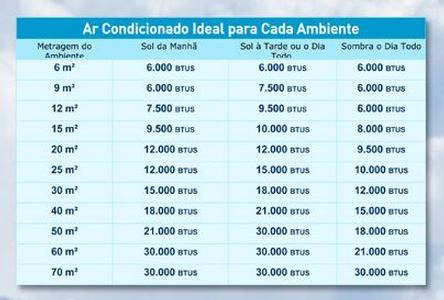
\includegraphics[width=\textwidth]{figuras/arcondicionado}
\end{figure}

\par Utilizando a metodologia de dimensionamento dos ar-condicionados presentes na casa chegou-se nos seguintes resultados:

\begin{table}
\centering
\captionof{table}{Aplicação do dimensionamento dos aparelhos de ar condicionado na casa modelo}
\begin{tabular}{|l|l|l|l|l|}
\hline
\multirow{\textbf{Cômodo}}  & \textbf{Área(m²)} & \textbf{N de pessoas} & \textbf{Aparelhos}    & \textbf{BTUs} \\
                            &                   &                       & \textbf{eletrônicos}  &               \\ \hline
Quarto 1 (Suite)            & 14,535 m²         & 2 pessoas             & 1                     & 10.000        \\ \hline
Quarto 2                    & 12,48 m²          & 2 pessoas             & 1                     & 9.000         \\ \hline
Sala                        & 9,585 m²          & 4 pessoas             & 2                     & 9.000         \\ \hline
Escritório                  & 9,6 m²            & 2 pessoas             & 1                     & 8.000         \\ \hline
\end{tabular}
\end{table}

\FloatBarrier
